% This file was created by matplotlib2tikz v0.5.3.
% The lastest updates can be retrieved from
% 
% https://github.com/nschloe/matplotlib2tikz
% 
% where you can also submit bug reports and leavecomments.
% 
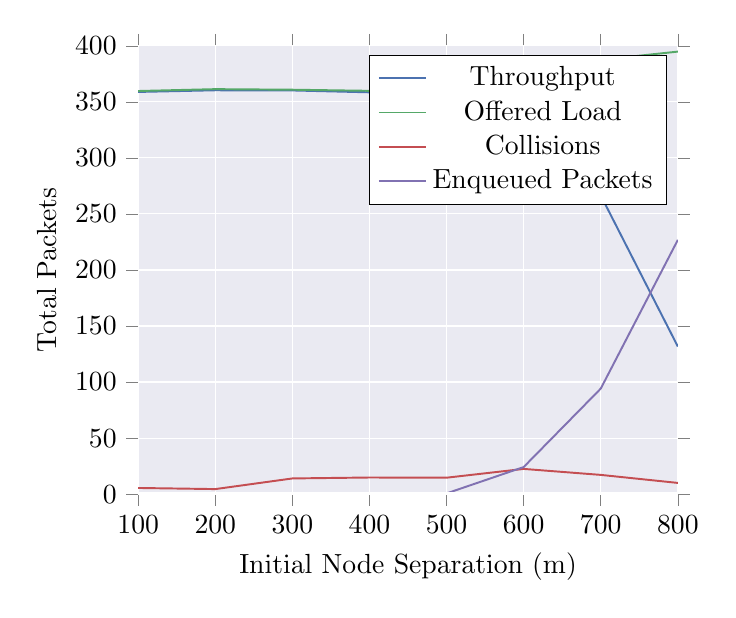
\begin{tikzpicture}

\definecolor{color1}{rgb}{0.298039215686275,0.447058823529412,0.690196078431373}
\definecolor{color0}{rgb}{0.917647058823529,0.917647058823529,0.949019607843137}
\definecolor{color3}{rgb}{0.768627450980392,0.305882352941176,0.32156862745098}
\definecolor{color2}{rgb}{0.333333333333333,0.658823529411765,0.407843137254902}
\definecolor{color4}{rgb}{0.505882352941176,0.447058823529412,0.698039215686274}

\begin{axis}[
xlabel={Initial Node Separation (m)},
ylabel={Total Packets},
xmin=100, xmax=800,
ymin=0, ymax=400,
xtick={100,200,300,400,500,600,700,800},
xticklabels={$100$,$200$,$300$,$400$,$500$,$600$,$700$,$800$},
ytick={0,50,100,150,200,250,300,350,400},
yticklabels={$0$,$50$,$100$,$150$,$200$,$250$,$300$,$350$,$400$},
tick align=outside,
xmajorgrids,
x grid style={white},
ymajorgrids,
y grid style={white},
axis line style={white},
axis background/.style={fill=color0},
legend entries={{Throughput},{Offered Load},{Collisions},{Enqueued Packets}}
]
\addplot [line width=0.7000000000000001pt, color1]
table {%
100 358.833333333333
200 360.333333333333
300 360.166666666667
400 358.5
500 359.166666666667
600 335.833333333333
700 266.5
800 131.666666666667
};
\addplot [line width=0.7000000000000001pt, color2]
table {%
100 359.666666666667
200 361.333333333333
300 360.833333333333
400 359.833333333333
500 362.666666666667
600 379
700 387.5
800 394.833333333333
};
\addplot [line width=0.7000000000000001pt, color3]
table {%
100 5.5
200 4.5
300 14
400 14.8333333333333
500 14.6666666666667
600 22.5
700 17.1666666666667
800 10
};
\addplot [line width=0.7000000000000001pt, color4]
table {%
100 0.166666666666667
200 0.666666666666667
300 0.166666666666667
400 0.166666666666667
500 0.666666666666667
600 24.1666666666667
700 94.1666666666667
800 226.833333333333
};
\path [draw=white, fill opacity=0] (axis cs:100,1)
--(axis cs:800,1);

\path [draw=white, fill opacity=0] (axis cs:1,0)
--(axis cs:1,400);

\path [draw=white, fill opacity=0] (axis cs:100,0)
--(axis cs:800,0);

\path [draw=white, fill opacity=0] (axis cs:0,0)
--(axis cs:0,400);

\end{axis}

\end{tikzpicture}